\begin{figure}[!h]
    \centering
    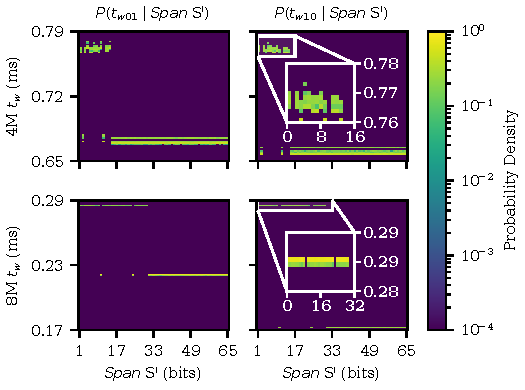
\includegraphics[width=0.95\linewidth]{fig/images/pdf/single-bit-sensitivity-scans-heat-bars-inset.pdf}
    \vspace{-.4cm}
    \caption{Write latency distributions for 1-bit $t_{w01}$ (left) and $t_{w10}$ (right) transitions within non-uniformly initialized 256-byte segments. Measurements from all 4 4M samples (top) and 4 8M samples (bottom) are aggregated. Each heatmap bar is a collapsed histogram colored according to the log-probability of observing a $t_w$ in each $\Delta t$-sized bin. The right plots zoom into the upper $t_w$ distributions to show 1-bit transitions that become \texttt{BIPOLAR} due to parity bit activity. \label{fig:sensitivity-scan}}
\end{figure}